\documentclass[tikz]{standalone}
\usetikzlibrary{calc,positioning,arrows}
\usepackage[T1]{fontenc} % Use 8-bit encoding that has 256 glyphs
\usepackage{fourier} % Use the Adobe Utopia font for the document - comment this line to return to the LaTeX default
\usepackage[english]{babel} % English language/hyphenation
\usepackage{amsmath,amsfonts,amsthm,stmaryrd} % Math packages
\usepackage{verbatim}
\begin{document}
	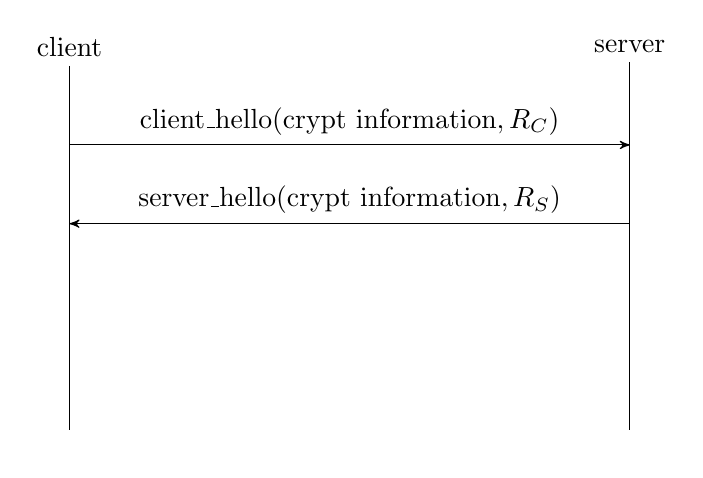
\begin{tikzpicture}[node distance=6cm,auto,>=stealth']
	\node[] (server) {server};
	\node[left = of server] (client) {client};
	\node[below of=server, node distance=5cm] (server_ground) {};
	\node[below of=client, node distance=5cm] (client_ground) {};
	%
	\draw (client) -- (client_ground);
	\draw (server) -- (server_ground);
	\draw[->] ($(client)!0.25!(client_ground)$) -- node[above,scale=1,midway]{$\text{client\_hello}(\text{crypt information},R_C)$} ($(server)!0.25!(server_ground)$);
	\draw[<-] ($(client)!0.45!(client_ground)$) -- node[above,scale=1,midway]{$\text{server\_hello}(\text{crypt information},R_S)$} ($(server)!0.45!(server_ground)$);
	\end{tikzpicture}
\end{document}